\documentclass[a4paper,10pt]{article}
\usepackage[utf8]{inputenc}
\usepackage[spanish,es-tabla]{babel}

\usepackage[a4paper,headheight=43pt,
            scale={0.8,0.8},hoffset=0.5cm,voffset=1cm]{geometry}

\usepackage{verbatim}

% paquetes matemáticos básicos
\usepackage{amsmath}
\usepackage{amsfonts}
\usepackage{amssymb}
\usepackage{xfrac}
\usepackage{siunitx}

% gráficos
\usepackage{graphicx}
\usepackage{float}
\usepackage{caption}
\usepackage{subfig}
\usepackage{listings}
\captionsetup[table]{font={small,sc},labelfont={small,sc}}

\usepackage[subrefformat=parens]{subcaption} % para colocar subfiguras con sus
                                             % respectivas referencias,
                                             % subrefformat es para que ponga
                                             % parentesis en las subref

\usepackage{appendix}
\usepackage[output-decimal-marker={,},per-mode=symbol-or-fraction,retain-unity-mantissa=true,detect-all,range-phrase={ -- },list-final-separator={ y }]{siunitx}
%output-decimal-marker define el separador decimal que se imprime
%per-mode define la forma que se utiliza para mostrar las unidades del denominador, en este caso elije segun el modo matematico que usa
%retain-unity-mantissa define si muestra o no la mantisa cuando es 1
%detect-all detecta la fuente que corresponde al entorno donde se colocan las unidades
%range-phrase define la palabra para los rangos de numeros
%list-final-separator define la palabra final de las listas

% paquete para insertar hipervínculos (sólo para el encabezado)
\usepackage[colorlinks=true,urlcolor=blue,
            linkcolor=black,linktoc=none,citecolor=black]{hyperref}

\usepackage[twoside]{fancyhdr}		% formato de página
\usepackage{lastpage}
% Configuración del encabezado y pie de página
\fancyhf{} % Limpia todos los campos de encabezado y pie de página
%\fancyhead[L]{\textbf{TB070 Dispositivos Semiconductores}}
\fancyfoot{} % Limpia el pie de página para personalizarlo a continuación

\fancyfoot[LE,RO]{\thepage/\pageref{LastPage}}
\fancyfoot[LE,RO]{\thepage/\pageref{LastPage}}

%*** redefino el comportamiento de los apendices
\renewcommand{\appendixname}{Apéndices}
\renewcommand{\appendixtocname}{Apéndices}
\renewcommand{\appendixpagename}{Apéndices}
%\renewcommand{\tablename}{Tabla}
%\renewcommand\spanishtablename{Tabla}
%\renewcommand{\figurename}{Figura}
%***
\pagestyle{fancy}

\usepackage[dvipsnames]{xcolor}
%\usepackage{todonotes}		% ToDo List
\usepackage{hyperref}		% formato de página
\usepackage{tcolorbox}

\DeclareSIUnit\angstrom{\text {Å}}

% \newif\ifturnotarde
% %     \turnotardetrue
% \newif\ifturnonoche
%     \turnonochetrue

\begin{document}

% Defino el formato del encabezado
%\pagestyle{fancy}
% \lhead{\includegraphics[width=0.3\textwidth]{lhead}}
% \chead{
%   {\scshape Dispositivos Semiconductores}\\
%   {\footnotesize 1\textsuperscript{er} cuatrimestre de 2023}
% }
%\rhead{\includegraphics[width=0.1\textwidth]{rhead}}
\lfoot{}
\cfoot{\thepage}
\rfoot{}
\begin{titlepage}

\thispagestyle{empty}

\begin{center}
    
\includegraphics[scale=0.3]{fiuba.pdf}\\
    \large{\textsc{Universidad de Buenos Aires}}\\
    \large{\textsc{Facultad de Ingeniería}}\\
    % Modificar año y cuatrimestre
    \small{Año 2026 - 2\textsuperscript{do} cuatrimestre}
\end{center}

\vfill
% Redefino la numeracion de las subsecciones
\renewcommand{\thesubsection}{\arabic{subsection}}

\begin{center}
	{\LARGE \underline{\textbf{Robótica industrial (TA155)}}}\\[0.5cm]
	{\LARGE \textbf{Trabajo Práctico 1 - Memoria Técnica:}}\\[0.5cm] 
    {\LARGE \textbf{Cinemática Inversa Numérica}}\\[0.5cm]
\end{center}

\begin{table}[H]
    \centering
    \begin{tabular}{|l|l|l|}
    \hline
    \multicolumn{3}{|c|}{\textbf{Integrantes}}    \\ \hline
    \multicolumn{1}{|l|}{Nombre y Apellido} & Padrón & Correo \\ \hline
    \multicolumn{1}{|l|}{Juan Ignacio Biancuzzo}    & 106005 & jbiancuzzo@fi.uba.ar \\ \hline
    \multicolumn{1}{|l|}{Rocio Nicole Heredia Piñon}   & 107621 & rherediap@fi.uba.ar \\ \hline
    \end{tabular}
\end{table}

\vfill

\end{titlepage}

\tableofcontents
\newpage


\section{Introducción}

Se busca a lo largo de este trabajo, resolver el problema de cinemática inversa del robot IRB140, de forma numérica y con un 100\% de acierto. Resolver el problema de cinemática inversa implica calcular las variables articulares necesarias para llevar al robot a la pose pedida. En principio, conociendo la pose de la herramienta, definida respecto de la terna de la base, se puede despejar $A_0^6$ para el problema de cinemática inverso como:

\begin{equation*}
    A_{0}^6 = (A_{base}^0)^{-1}POSE(A_6^{tool})^{-1}
\end{equation*}

Luego, conociendo $A_0^6$, definida como la pose de la terna 6 respecto de la terna 0, se despeja $\mathbf{q}$. La idea es no plantearlo de forma analítica, sino de forma numérica. Se conoce que la solución depende de la configuración elegida del robot, dado que hay varias formas para llegar a una misma pose. Por lo que no solo se aclara la pose, sino también la configuración del robot para resolver el problema de cinemática inverso. 

Al plantearlo de forma numérica, se encara el problema partiendo desde un conjunto de variables articulares iniciales, una semilla. La idea será plantear el problema de cinemática directa, que dará la pose de la herramienta con estos valores articulares, y evaluar qué tan lejos está la pose calculada de la pose destino. Luego, $\mathbf{q}$ se mueve de forma tal que ese error disminuya. De esta forma, es necesario un algoritmo que calcule la pose de la herramienta a partir de $\mathbf{q}$. 

\subsection{Cinemática directa}

Para resolver el problema de cinemática directa, se comienza reconociendo los eslabones y ejes que conforman el robot IRB140. Luego, se definen las ternas asociadas a cada uno siguiendo las reglas de Denavit-Hartemberg. Esta asignación se muestra en la figura \ref{fig:ternas_irb140}.

\begin{figure}[H]
    \centering
    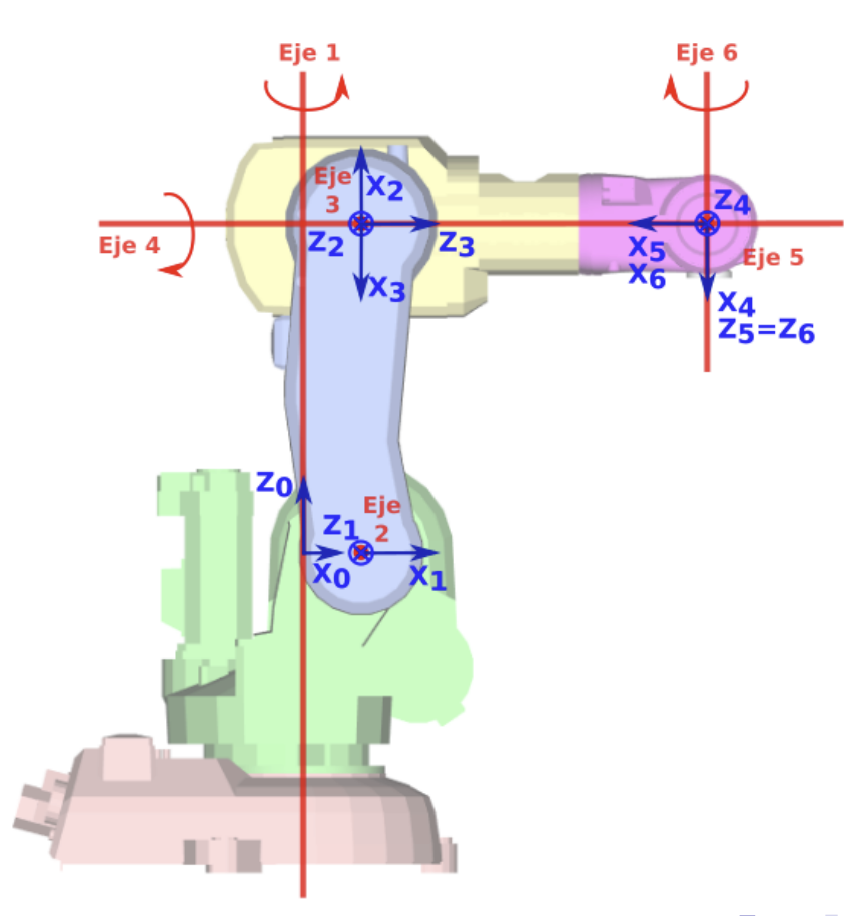
\includegraphics[width=0.5\linewidth]{imagenes/irb140_ternas.png}
    \caption{Asignación de ternas del robot IRB140.}
    \label{fig:ternas_irb140}
\end{figure}

Otro criterio tenido en cuenta para la asignación de ternas fue, en la medida de lo posible, simplificar el problema de cinemática directa anulando algunos parámetros DH. Entre estos parámetros se encuentran la rotación de la articulación $i$ ($\theta_i$), la longitud de la articulación $i$ ($\text{d}_i$), la longitud del eslabón $i$ ($\text{a}_i$) y la torsión del eslabón $i$ ($\alpha_i$). La idea es que para llevar la terna $i-1$ a la terna $i$, esta debe sufrir una serie de transformaciones asociadas a estos parámetros. En primer lugar, se rota la terna $i-1$ alrededor de su eje $z_{i-1}$ hasta alinear $x_{i-1}$ con $x_i$. Este ángulo de rotación es $\theta_i$. Luego, se desplaza la terna rotada en $z_{i-1}$ hasta llevar su origen sobre la recta que corta perpendicularmente a los ejes $i$ e $i+1$. La cantidad que se desplaza es $\text{d}_i$. Luego, esta terna ya rotada y trasladada, se desplaza en $x_i$ rotado, hasta hacer coincidir su origen con el de la terna $i$. Este desplazamiento es en $\text{a}_i$. Finalmente, se realiza una última rotación alrededor de $x_i$ para que la terna coincida completamente con la terna $i$. Esta última rotación se realiza en un ángulo $\alpha_i$. Sabiendo cómo plantear las transformaciones de una terna a la siguiente se puede calcular su matriz de rototraslación como:

\begin{equation*}
    A_{i-1}^i = R(z, \theta_i)T(z, d_i)T(x, a_i)R(x, \alpha_i) = 
    \begin{pmatrix}
        c\theta_i & -s\theta_ic\alpha_i & s\theta_is\alpha_i & \text{a}_ic\theta_i \\
        s\theta_i & c\theta_ic\alpha_i & -c\theta_is\alpha_i & \text{a}_is\theta_i \\
        0 & s\alpha_i & c\alpha_i & \text{d}_i \\
        0 & 0 & 0 & 1
    \end{pmatrix}
\end{equation*}


Además, estas transformaciones permiten entender cómo se definen los parámetros DH, para así calcularlos en este robot particular. La tabla de parámetros DH es la \ref{tab:parametros_irb140}, donde se utilizan constantes asociadas a la geometría del robot que pueden observarse en la figura \ref{fig:param_irb140}. 

\begin{figure}[H]
    \centering
    \begin{minipage}[c]{0.48\textwidth}
        \centering
        \begin{tabular}{|c|c|c|c|c|}
        \hline
             & $\theta$ & $\text{d}$ & $\text{a}$ & $\alpha$ \\ \hline
           1 & $q_1$ & 0 & $\text{a}_1$ & $-\pi/2$ \\ \hline
           2 & $q_2$ & 0 & $\text{a}_2$ & 0 \\ \hline
           3 & $q_3$ & 0 & 0 & $\pi/2$ \\ \hline
           4 & $q_4$ & $\text{d}_4$ & 0 & $-\pi/2$ \\ \hline
           5 & $q_5$ & 0 & 0 & $\pi/2$ \\ \hline
           6 & $q_6$ & 0 & 0 & 0 \\ \hline
        \end{tabular}
        \captionof{table}{Tabla de parámetros DH para IRB140.}
        \label{tab:parametros_irb140}
    \end{minipage}
    \hfill
    \begin{minipage}[c]{0.48\textwidth}
        \centering
        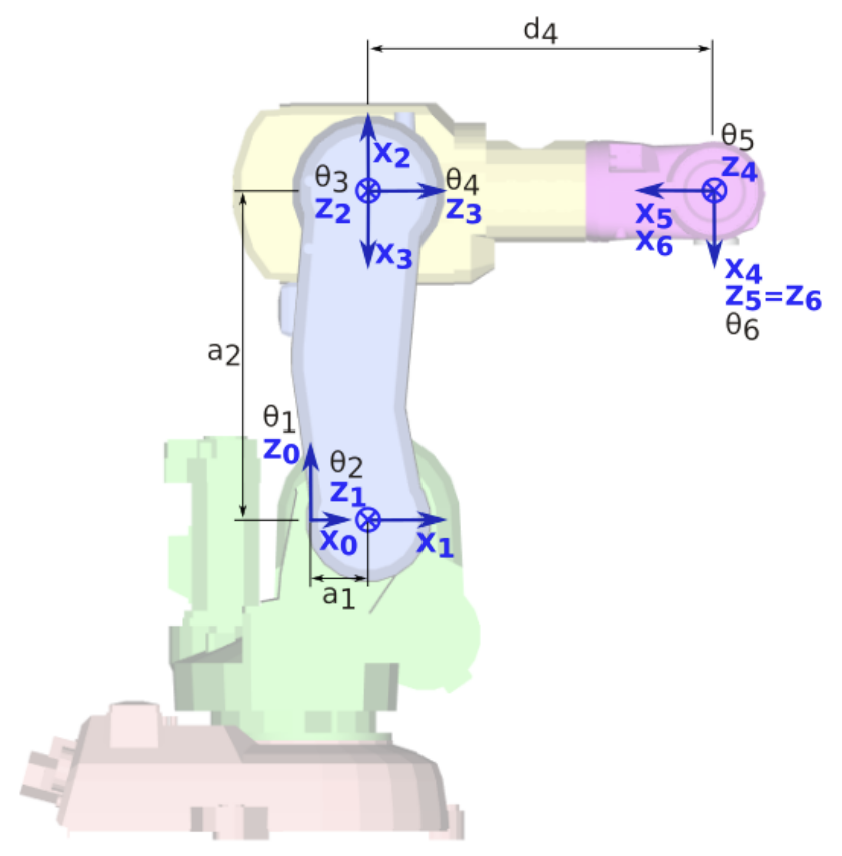
\includegraphics[width=\linewidth]{imagenes/irb140_dh.png}
        \captionof{figure}{Parámetros de DH del IRB140.}
        \label{fig:param_irb140}
    \end{minipage}
\end{figure}

En el caso particular del robot IRB140, las constantes $\text{a}_1$, $\text{a}_2$ y $\text{d}_4$ están dadas por:

\begin{equation*}
    \begin{cases}
        \text{a}_1 = \SI{70}{\milli\meter} \\
        \text{a}_2 = \SI{360}{\milli\meter}\\
        \text{d}_4 = \SI{380}{\milli\meter}
    \end{cases}
\end{equation*}

Conociendo los parámetros, se pueden armar las matrices de rototraslación $A_0^1$, $A_1^2$, $A_2^3$, $A_3^4$, $A_4^5$ y $A_5^6$ con la forma genérica previamente planteada. Y finalmente, calcular $A_0^6$ a partir del producto de estas matrices:

\begin{equation*}
    A_0^6 = A_0^1A_1^2A_2^3A_3^4A_4^5A_5^6
\end{equation*}

Sin embargo, cuando se habla de pose del robot, uno se refiere a la pose de la herramienta definida respecto de la base del robot. Se necesita un último cálculo para encontrarla:

\begin{equation*}
    POSE = A_{base}^0A_0^6A_6^{tool}
\end{equation*}

Donde $A_{base}^0$ y $A_6^{tool}$ se definirán según cómo se toma la terna de la base y la terna de la herramienta siguiendo las mismas transformaciones ya planteadas. 

El algoritmo desarrollado para resolver el problema de cinemática directa realiza este mismo procedimiento. Se define una función que calcula las matrices de rototraslación a partir de los parámetros de DH y se utiliza para calcular cada matriz en particular según los parámetros definidos en la tabla y según las variables articulares tomadas. Luego, calcula la pose a partir del producto de matrices, considerando además las matrices de rototraslación desde la base a la terna 0 y desde la terna 6 a la terna $tool$. 

\section{Algoritmo para el problema cinemático inverso}

\subsection{Solución 1: no se consideran las configuraciones}

En un principio, se plantea el algoritmo de forma tal que encuentre un conjunto $\mathbf{q}$ que logre llevar la herramienta a la pose deseada, pero no necesariamente en la configuración pedida. La idea del algoritmo es la misma que se planteó en la introducción. Se parte de un set de variables articulares inicial y se calcula la pose definida a partir de estas planteando el problema de cinemática directo. Luego, se evalúa qué tan alejadas están las poses entre sí y se plantea un nuevo vector de variables articulares para acercar la pose a la deseada. De esta forma, el primer paso consiste en definir $\mathbf{q}_{\text{semilla}}$, en principio de manera aleatoria. Esto da comienzo al algoritmo iterativo, que finaliza al encontrar la solución o al llegar a un máximo de iteraciones definido. Este se puede plasmar paso a paso de la siguiente manera:

\begin{itemize}
    \item \textbf{Paso 1}: se toma el vector $\mathbf{q}_{i-1}$ calculado en la iteración anterior (o la semilla en el caso de ser la primera iteración) y se calcula la pose de la herramienta en base a cómo está articulado el robot ($POSE_i$). Esto es resolver justamente el problema de cinemática directa. 
    \item \textbf{Paso 2}: se evalúa que tan lejos está la pose actual de la pose destino. Esto da una idea de qué tan buena solución es $\mathbf{q}_{i-1}$ para el problema de cinemática inversa. Este $\Delta POSE$ no se puede plantear simplemente como una resta de poses, que en el problema de cinemática directa se definen como matrices de rototraslación. Se puede dividir el problema y comparar por separado la diferencia en la traslación y en la orientación de las poses. Para la traslación, se puede plantear directamente la resta entre los vectores de traslación que definen a cada pose:

    \begin{equation*}
        \delta \mathbf{p}^{base} = \mathbf{p}_{base, tool~final}^{base} - \mathbf{p}_{base, tool~i}^{base}
    \end{equation*}

    Para la orientación, se puede analizar la rotación necesaria para llegar de una orientación a la otra, que da una idea de qué tan alejadas están entre sí:

    \begin{equation*}
        R^{tool~final}_{base} = R_{base}^{tool~i}R_{tool~i}^{tool~final}
    \end{equation*}

    De esta forma, se puede despejar $R_{tool~i}^{tool~final}$ como:

    \begin{equation*}
        R_{tool~i}^{tool~final} = (R_{base}^{tool~i})^TR^{tool~final}_{base}
    \end{equation*}

    Esta rotación, que se describe a través de la matriz, se puede también representar a través de un vector $\mathbf{k}$ y un ángulo de rotación $\theta$. O incluso un vector $\delta\boldsymbol{\theta} = \theta\mathbf{k}$. Este se utiliza para indicar la diferencia entre orientaciones, que sería distinto a restar directamente los vectores asociados a la orientación final y la actual. Sin embargo, es necesario tener en cuenta que este vector indica el eje de rotación y el ángulo para llevar de una orientación a otra respecto de la terna $i$. Con una matriz de cambio de base, podemos representar este vector respecto de la base, así como representamos los vectores de traslación: 

    \begin{equation*}
        \boldsymbol{\theta}^{base} = R_{base}^{tool ~ i}\boldsymbol{\theta}^{tool~i}
    \end{equation*}

    El problema inverso que permite calcular $\mathbf{k}$ y $\theta$ a partir de una matriz de rotación se resuelve en el Anexo \ref{sec:problema_inverso}.
    
    Finalmente, se construye $\Delta POSE$ como:

    \begin{equation*}
        \Delta POSE = 
        \begin{pmatrix}
            \delta \mathbf{p}^{base}\\
            \delta \boldsymbol{\theta}^{base}
        \end{pmatrix}
    \end{equation*}

    Este vector da una idea de la dirección en la que debería moverse el robot para llegar a la pose deseada desde la pose actual en línea recta. Aunque la problemática en este caso no es mover el robot desde una pose inicial a una final, en cuanto al algoritmo la idea es similar. Se busca que la pose se vaya acercando a la final a medida que se avanza en las iteraciones, y una forma de que lo haga es en esta línea recta.

    \item \textbf{Paso 3}: para acercarse a la pose deseada, se puede avanzar en la dirección que indica $\Delta POSE$, como se mencionó previamente. Se puede plantear avanzar en un pequeño paso, $\delta POSE$, que se relaciona con $\Delta POSE$ de manera directa como:

    \begin{equation*}
        \delta POSE = \alpha \Delta POSE
    \end{equation*}

    Con $\alpha$ un número pequeño. Se conoce, además, que hay una relación entre la velocidad del robot y la velocidades articulares a través del Jacobiano:

    \begin{equation*}
        \begin{cases}
            \mathbf{v} = J_v\mathbf{\dot{q}} \\
            \boldsymbol{\omega} = J_{w}\mathbf{\dot{q}}
        \end{cases}
    \end{equation*}

    Considerando a las velocidades derivadas de las posiciones, se puede realizar la siguiente aproximación para pequeños desplazamientos:

    \begin{equation*}
        \frac{\delta \mathbf{p}}{\delta t} = J_v\frac{\delta \mathbf{q}}{\delta t}
    \end{equation*}

    \begin{equation*}
        \frac{\delta \boldsymbol{\theta}}{\delta t} = J_w\frac{\delta \mathbf{q}}{\delta t}
    \end{equation*}

    De esta forma, se puede calcular de forma aproximada el pequeño desplazamiento en la pose del robot ante una pequeña variación de sus valores articulares como:

    \begin{equation*}
        \delta POSE = J\delta \mathbf{q}
    \end{equation*}

    En este caso, es de interés despejar $\delta \mathbf{q}$:

    \begin{equation*}
        \delta\mathbf{q} = J^+ \delta POSE
    \end{equation*}

    Donde $J+$ es la pseudo-inversa del Jacobiano. Como será necesaria, en este paso se calculan el Jacobiano y su pseudo-inversa. Planteando las velocidades de la terna 6, descripta respecto de la misma terna 6, el Jacobiano se puede plantear de forma genérica como:

    \begin{equation*}
        J_{o6}^6 = 
        \begin{pmatrix}
            (\mathbf{p}_{0,6}^0 \times \mathbf{x}_6^0)\Big|_z & (\mathbf{p}_{1,6}^1 \times \mathbf{x}_6^1)\Big|_z & (\mathbf{p}_{2,6}^2 \times \mathbf{x}_6^2)\Big|_z & (\mathbf{p}_{3,6}^3 \times \mathbf{x}_6^3)\Big|_z & (\mathbf{p}_{4,6}^4 \times \mathbf{x}_6^4)\Big|_z & (\mathbf{p}_{5,6}^5 \times \mathbf{x}_6^5)\Big|_z \\
            
            (\mathbf{p}_{0,6}^0 \times \mathbf{y}_6^0)\Big|_z & (\mathbf{p}_{1,6}^1 \times \mathbf{y}_6^1)\Big|_z & (\mathbf{p}_{2,6}^2 \times \mathbf{y}_6^2)\Big|_z & (\mathbf{p}_{3,6}^3 \times \mathbf{y}_6^3)\Big|_z & (\mathbf{p}_{4,6}^4 \times \mathbf{y}_6^4)\Big|_z & (\mathbf{p}_{5,6}^5 \times \mathbf{y}_6^5)\Big|_z \\
            
            (\mathbf{p}_{0,6}^0 \times \mathbf{z}_6^0)\Big|_z & (\mathbf{p}_{1,6}^1 \times \mathbf{z}_6^1)\Big|_z & (\mathbf{p}_{2,6}^2 \times \mathbf{z}_6^2)\Big|_z & (\mathbf{p}_{3,6}^3 \times \mathbf{z}_6^3)\Big|_z & (\mathbf{p}_{4,6}^4 \times \mathbf{z}_6^4)\Big|_z & (\mathbf{p}_{5,6}^5 \times \mathbf{z}_6^5)\Big|_z \\

            \mathbf{x}^0_6\big|_z &\mathbf{x}^1_6\big|_z & \mathbf{x}^2_6\big|_z & \mathbf{x}^3_6\big|_z & \mathbf{x}^4_6\big|_z & \mathbf{x}^5_6\big|_z \\

            \mathbf{y}^0_6\big|_z &\mathbf{y}^1_6\big|_z & \mathbf{y}^2_6\big|_z & \mathbf{y}^3_6\big|_z & \mathbf{y}^4_6\big|_z & \mathbf{y}^5_6\big|_z \\

            \mathbf{z}^0_6\big|_z &\mathbf{z}^1_6\big|_z & \mathbf{z}^2_6\big|_z & \mathbf{z}^3_6\big|_z & \mathbf{z}^4_6\big|_z & \mathbf{z}^5_6\big|_z \\
        \end{pmatrix}
    \end{equation*}

    Esta representación genérica proviene del mecanismo del robot con 6 articulaciones de revolución, utilizando el concepto de cinemática de un cuerpo rígido. Estos vectores se pueden calcular fácilmente a partir del problema de cinemática directa. Los vectores $\mathbf{x}_6^i$, $\mathbf{y}_6^i$ y $\mathbf{z}_6^i$ son los vectores columna de la matriz de rotación $R_j^6$ y los vectores $\mathbf{p}_{i,6}^i$ son los vectores de traslación de las matrices $A_i^6$. Es decir, conociendo $A_0^6$, $A_1^6$, $A_2^6$, $A_3^6$, $A_4^6$ y $A_5^6$, se puede calcular el Jacobiano. Sin embargo, cuando se plantea $\delta POSE$, se está calculando en la terna $tool$ y respecto de la terna $base$. Se puede plantear el Jacobiano $J_{tool}^{base}$ siguiendo la forma genérica o aún más simple, se plantea el cambio de terna y el cambio de punto de cálculo como:

    \begin{equation*}
        J_{tool}^{base} = 
        \begin{pmatrix}
            R_{base}^6 & -R_{base}^6[\mathbf{p}_{6,tool}^6]_{\times} \\
            0_{3\times 3} & R_{base}^6
        \end{pmatrix}
        J_{o6}^6
    \end{equation*}

    Donde $[\mathbf{p}_{6,tool}^6]_{\times}$ es la matriz antisimétrica dada por:

    \begin{equation*}
        [\mathbf{k}]_{\times} = 
        \begin{pmatrix}
            0 & -k_z & k_y \\
            k_z & 0 & -k_x \\
            -k_y & k_x & 0
        \end{pmatrix}
    \end{equation*}
    
    El cambio de base se plantea directo con las matrices de rotación y el cambio de punto de cálculo se plantea relacionando las velocidades de dos puntos dentro de un mismo cuerpo rígido. 

    Finalmente, una vez construido el Jacobiano, se calcula su pseudo-inversa como:

    \begin{equation*}
        J^+ = (J^TJ)^{-1}J^T
    \end{equation*}

    Es conveniente utilizar la pseudo-inversa en vez de la inversa considerando que el Jacobiano no siempre es cuadrado, y muchas veces, aunque lo sea, en una configuración singular puede perder rango. En este caso, sí es cuadrada excepto que se evalúe en una configuración donde tenga un rango menor a 6. 

    \item \textbf{Paso 4}: con el Jacobiano ya calculado, se calcula la variación de los valores articulares que corresponden al pequeño desplazamiento en dirección a la pose final:

    \begin{equation*}
        \delta \mathbf{q} = \alpha J^+\Delta POSE 
    \end{equation*}    

    Se calcula entonces un nuevo $\mathbf{q}_i$ como:

    \begin{equation*}
        \mathbf{q}_i = \mathbf{q}_{i-1} + \delta\mathbf{q} = \mathbf{q}_{i-1} + \alpha J^+\Delta POSE
    \end{equation*}

    Este $\mathbf{q}_i$ llevaría a la pose del robot más cerca de la pose destino en cada iteración, hasta que, idealmente, llegaría a la pose deseada y el $\mathbf{q}$ sería el valor de articulaciones final que logra esta misma pose. 
\end{itemize}

\subsubsection{Pruebas}
Se llevó a cabo un número de pruebas para confirmar el funcionamiento de esta solución, buscando confirmar el objetivo de una capacidad de aciertos del $100\%$.

Para esto se generaron $N$ valores de $\mathbf{q}$, de los cuales se filtraron aquellos que estén cerca de una singularidad, para obtener variables articulares las cuales sean alcanzables por un método iterativo como este y muestre las virtudes y defectos de la solución propuesta, y no fallas por valores numéricos difícilmente alcanzables. Se logró crear este filtrado por medio de establecer una cota inferior a la manipulabilidad $W(\mathbf{q})$ la cual se detalla en el Anexo \ref{sec:manipulabilidad}.

Se ejecutaron las pruebas para $N = 100$, y se obtuvo aproximadamente un $10\%$ de aciertos. A pesar que este resultado sea el esperado, se vuelve valioso analizar porque se obtuvo un resultado tan bajo, para plantear una nueva solución. 

Analizando un caso fallido, como el siguiente:
\begin{verbatim}
Deseada: [ 0.307  1.352  0.646  0.282 -0.48   0.917]
Obtenida: [ 0.306  1.405  0.542 -2.865  0.413 -2.269]
Pose deseada: Pose(
    rotacion = [
        [-0.149, -0.101,  0.984],
        [ 0.91 ,  0.375,  0.177],
        [-0.387,  0.921,  0.036]], 
    translacion = [ 0.471,  0.149, -0.157]
)
Pose obtenida: Pose(
    rotacion = [
        [-0.167, -0.103,  0.98 ],
        [ 0.889,  0.415,  0.195],
        [-0.427,  0.904,  0.022]], 
    translacion = [ 0.46 ,  0.146, -0.143]
)
\end{verbatim}
se notó que tanto la rotación como la translación, aunque levemente distintos, representarían que la pose deseada y la pose obtenida son la misma, pero al obtenerse valores articulares distintos queda en evidencia que cada $\mathbf{q}$ perteneces a configuraciones distintas que resultan en la misma pose con lo que deberíamos plantear una solución que tenga en cuenta la configuración de la pose deseada.

\subsection{Solución 2: se inicializa la semilla en la configuración deseada}

La solución previamente planteada hizo evidente que se debe tener en cuenta la configuración deseada en el desarrollo del algoritmo. Si se llega a la pose destino pero no en la configuración pedida, el $\mathbf{q}$ resultante no es correcto. Y si no se tiene en cuenta, la configuración depende mucho de la semilla que se utilice y sería una casualidad que llegue justo en al configuración que se pide. Por esta razón, se plantea inicializar la semilla ya en la configuración deseada, aumentando las chances de que encuentre una trayectoria hacia la pose destino sin cambiar de configuración. Sin embargo, este método no lo asegura. Para esto, se plantean las 3 configuraciones posibles del robot. $\text{conf}_1$ está asociado al brazo hacia adelante ($1$) y brazo hacia atrás ($-1$) y se puede calcular como:

\begin{equation*}
    \text{conf}_1 = \text{sign}(d_4s_{23}+a_2c_2+a_1)
\end{equation*}

Si $d_4s_{23}+a_2c_2+a_1$, se tiene una situación de singularidad, en la cual la muñeca cruza el eje 1. 

$\text{conf}_2$ está asociado con las configuraciones codo positivo ($1$) y codo negativo ($-1$) y se puede calcular como:

\begin{equation*}
    \text{conf}_2 = \text{sign}(c_3)
\end{equation*}

Si $c_3 = 0$, que sucede con $q_3 = \pm \frac{\pi}{2}$, entonces se tiene una configuración singular en la cual el brazo esta extendido o plegado. 

$\text{conf}_3$ está asociado con las configuraciones de la muñeca, positiva ($1$) y negativa ($-1$), que se calcula directamente como:

\begin{equation*}
    \text{conf}_3 = \text{sign}(q_5)
\end{equation*}

Si $q_5 = 0$, se tiene una configuración singular donde quedan alineados los ejes 4 y 6.

Es posible notar que el hecho de conocer las configuraciones da información sobre los valores posibles que pueden tomar $q_2$, $q_3$ y $q_5$ para lograr una pose en la configuración deseada. Además, en los cambios de configuración, el robot se encuentra en una situación de singularidad donde el Jacobiano pierde rango. De esta forma se puede armar la semilla fijando $q_2$, $q_3$ y $q_5$ para que arranque en la configuración pedida. Para esto se pueden considerar las siguientes relaciones:

\begin{equation*}
    \cos(q_3) > 0
\end{equation*}

\begin{equation*}
    -\pi/2<q_3<\pi/2
\end{equation*}

Por lo que se puede elegir $q_3$ entre $-\pi/2$ y $\pi/2$ si la $\text{conf}_2$ es 1, sino se elige por fuera de este intervalo (manteniendo que sea un valor entre $-\pi$ y $\pi$). 

Luego, para la tercer configuración se puede plantear directamente que se elige $q_5>0$ si $\text{conf}_3 = 1$ y $q_5<0$ si $\text{conf}_3 = -1$.

Para el caso de $\text{conf}_1$, si $q_3 = 0$ se puede plantear:

\begin{equation*}
    a_1 + a_2\cos(q_2) + d_4\sin(q_2) \gtrless 0
\end{equation*} 

En el caso en el que $\text{conf}_1 = -1$, se podría buscar el $q_2$ que minimiza la expresión. Esta expresión también se puede plantear como:

\begin{equation*}
    \frac{a_1}{k} + \frac{a_2}{k}\cos(q_2) + \frac{d_4}{k}\sin(q_2) \gtrless 0
\end{equation*}

Donde $k = \sqrt{a_2^2 + d_4^2}$. 

\begin{equation*}
    \frac{a_1}{k} + \sin\left(q_2 + \arctan\left(\frac{a_2}{d_4} \right)\right) \gtrless 0
\end{equation*}

Como $\frac{a_1}{k}>0$, el $q_2$ que minimiza la expresión es aquel para el cual:

\begin{equation*}
    \sin\left(q_2 + \arctan\left(\frac{a_2}{d_4} \right) \right) = -1
\end{equation*}

\begin{equation*}
    q_2 + \arctan\left(\frac{a_2}{d_4} \right) = -\frac{\pi}{2}
\end{equation*}

\begin{equation*}
    q_2 = -\frac{\pi}{2} - \arctan\left(\frac{a_2}{d_4} \right) = \arctan\left(\frac{d_4}{a_2} \right) - \pi
\end{equation*}

Podría ser que $q_2$, por más que lleve al mínimo del argumento, no lo haga negativo. Pero en ese caso, no se podría lograr nunca esta configuración. 

Si $q_3 = \pi$, la idea es la misma solo que se invierte la solución para $\text{conf}_1 = -1$:

\begin{equation*}
    q_2 = \pi - \arctan\left(\frac{d_4}{a_2} \right)
\end{equation*}

Luego, si quiero plantear $\text{conf}_1 = 1$, puedo buscar un $q_2$ que haga que el argumento sea positivo, es decir:

\begin{equation*}
    \frac{a_1}{k} + \sin\left(q_2 + \arctan\left(\frac{a_2}{d_4} \right)\right) > 0
\end{equation*}

Como $\frac{a_1}{k}>0$, se podría plantear que:

\begin{equation*}
    \sin\left(q_2 + \arctan\left(\frac{a_2}{d_4} \right)\right) > 0
\end{equation*}

Asimismo, $0<\arctan\left(\frac{a_2}{d_4} \right)<\frac{\pi}{2}$, por lo que si se toma $q_2 = 0$, siempre se va a cumplir que el argumento se hace positivo. Esto es válido para $q_3 = 0$ y para $q_3 = \pi$. 

Finalmente se considera que:

\begin{equation*}
    \begin{cases}
        \text{conf}_2 = 1\rightarrow q_3 = 0\\
        \text{conf}_2 = -1\rightarrow q_3 = \pi\\
        \text{conf}_3 = 1\rightarrow q_5 = \pi / 2\\
        \text{conf}_3 = -1\rightarrow q_5 = -\pi / 2\\
        \text{conf}_1 = 1 \rightarrow q_2 = 0 \\
        \text{conf}_1 = -1\rightarrow q_2 = 
        \begin{cases}
            \arctan\left(\frac{d_4}{a_2} - \pi \right) ~\text{si} ~ q_3 = 0 \\
            \pi - \arctan\left(\frac{d_4}{a_2}\right) ~\text{si} ~ q_3 = \pi
        \end{cases}
    \end{cases}
\end{equation*}

Se plantea esto de forma genérica, buscando que sea válido incluso si cambian $a_1$, $a_2$ o $d_4$. 

El algoritmo sigue exactamente la misma lógica que antes, en esta solución solo se plantea que la semilla arranque en la configuración pedida. Sin embargo, el hecho de que arranque en esta configuración no impide que para llegar a la pose final encuentre una solución cambiando de configuración. Puede que la trayectoria recta entre la pose actual y la pose final que plantea de alguna manera el algoritmo pase por una singularidad, o cerca de ella. Para evitar esta situación, se plantea una nueva solución, donde se contempla la posibilidad de que la configuración cambie y ante esa situación, se modifique la semilla. 

\subsubsection{Pruebas}
Nuevamente se ejecutaron las pruebas para $N = 100$, y se obtuvo aproximadamente un $85\%$ donde se pudo notar que nuestra conclusión sobre utilizar información de la configuración para determinar la semilla inicial, le permite a la solución encontrar las variables articulares deseadas.

Por otro lado, de las pruebas fallidas se detectó que ninguna mantuvo la configuración de la semilla, por lo que el error no venía por una diferencia de la pose sino por encontrar una solución que tenga otra configuración. De forma similar a la solución anterior, se debe incorporar más información a la semilla para obtener un porcentaje de aciertos del $100\%$ y ya habiendo determinado los valores de $q_2$, $q_3$ y $q_5$ por la configuración, se necesita incorporar información sobre $q_1$, $q_4$ y $q_6$.

\subsection{Solución 3: se inicializa la semilla en la configuración deseada y se contempla que se mantenga en ella}

Como bien se comentó previamente, puede que una semilla se inicialice en la configuración correcta pero que el algoritmo encuentre una trayectoria hacia la pose deseada en la cual se debe cambiar de configuración para llegar. Para evitar esta situación, se debe proveer más información para inicializar la semilla correctamente. Como la configuración deseada da información acerca de $q_2$, $q_3$ y $q_5$, se necesita información acerca de $q_1$, $q_4$ y $q_6$ para que la semilla se inicialice asociada a una pose cercana a la final, que no requiera pasar por singularidades para alcanzarla. De esta forma, se debe dar de dato al algoritmo los cuadrantes donde se desea que estén ubicados los ejes 1, 4 y 6. Se incorpora esta nueva información para la inicialización de la semilla, y en el caso en el cual se detecte un cambio de configuración, se la vuelve a inicializar tomando otros valores para $q_1$, $q_4$ y $q_6$, respetando los cuadrantes dados y con un límite particular de intentos. Cuando se vuelve a inicializar la semilla, se reinicia la cantidad de iteraciones, para darle tiempo a que el algoritmo converja. 

En el caso que no se sepan los cuadrantes en los que se encuentran $q_1$, $q_4$ y $q_6$, se puede plantear esta misma idea, solo que se debería probar inicializar la semilla cambiando también los cuadrantes. Llevaría más iteraciones y por ende más tiempo pero se lograría llegar a la solución correcta. 

\subsubsection{Pruebas}
Finalmente, se ejecutaron las pruebas para $N = 1000$ y se obtuvo un $100\%$ de aciertos donde demuestra que la información faltante era sobre los cuadrantes de $q_1$, $q_4$ y $q_6$, incorporando la posibilidad de reintentar en el caso de cambiar de configuración.

Cabe remarcar que a pesar de conseguir un $100\%$ de aciertos no significa que para cualquier valor de $\alpha$, cantidad de reintentos e iteraciones se llegue a la solución correcta, sino que estos hiperparámetros necesitan ser elegidos correctamente para asegurar la solución correcta. 

\newpage

\section{Anexo}

\subsection{Solución al problema inverso de la rotación eje-ángulo}
\label{sec:problema_inverso}

La matriz que representa la rotación alrededor de un eje $\mathbf{k}$ en $\theta$ se puede escribir como:

\begin{equation*}
    R(\mathbf{k}, \theta) = 
    \begin{pmatrix}
        k_xk_x(1-\cos(\theta))+\cos(\theta) & k_xk_y(1-\cos(\theta)) & k_xk_z(1-\cos(\theta)) \\
        k_xk_y(1-\cos(\theta)) & k_yk_y(1-\cos(\theta))+\cos(\theta) & k_yk_z(1-\cos(\theta)) \\
        k_xk_z(1-\cos(\theta)) & k_yk_z(1-\cos(\theta)) & k_zk_z(1-\cos(\theta))+\cos(\theta)
    \end{pmatrix} 
    +
\end{equation*}
\begin{equation*}
        +
    \begin{pmatrix}
        0 & -k_z\sin(\theta) & k_y\sin(\theta) \\
        k_z\sin(\theta) & 0 & -k_x\sin(\theta) \\
        -k_y\sin(\theta) & k_x\sin(\theta) & 0
    \end{pmatrix} = 
    \begin{pmatrix}
        r_{11} & r_{12} & r_{13} \\
        r_{21} & r_{22} & r_{23} \\
        r_{31} & r_{32} & r_{33}
    \end{pmatrix}
\end{equation*}

Se puede utilizar la traza de la matriz para despejar $\cos(\theta)$: 

\begin{equation*}
    \cos(\theta) = \frac{\text{tr}(R(\mathbf{\mathbf{k}}, \theta))-1}{2}
\end{equation*}

$\mathbf{k}$ se puede plantear como:

\begin{equation*}
    \mathbf{k} = 
    \begin{pmatrix}
        k_x \\
        k_y \\
        k_z
    \end{pmatrix}
    =
    \begin{pmatrix}
        \frac{r_{32}-r_{23}}{2\sin(\theta)} \\
        \frac{r_{13}-r_{31}}{2\sin(\theta)} \\
        \frac{r_{21}-r_{12}}{2\sin(\theta)}
    \end{pmatrix}
\end{equation*}

Conociendo $\cos(\theta)$ se tendrían dos soluciones para $\theta$ pero es lo mismo tener $R(\mathbf{k}, \theta)$ o $R(-\mathbf{k}, -\theta)$. Por lo que se puede despejar directamente con $\arccos$. 

Esta solución trae problemas cuando $\sin(\theta) = 0$, ya sea porque $\theta= 0$ o porque $\theta = \pm \pi$ (considerando que $\theta$ se mantiene entre $-\pi$ y $\pi$). Si $\theta = 0$, no se está rotando, se tendría que la matriz es la identidad. Por lo que directamente $\mathbf{k}$ podría ser cualquier vector, manteniendo $\theta = 0$. Cuando $\theta = \pm \pi$, la matriz se simplifica como:

\begin{equation*}
    R(\mathbf{k}, \theta) =
    \begin{pmatrix}
        2k_x^2-1 & 2k_xk_y & 2k_xk_z \\
        2k_xk_y & 2k_y^2-1 & 2k_yk_z \\
        2k_xk_z & 2k_yk_z & 2k_z^2-1
    \end{pmatrix}
\end{equation*}

De esta forma, es posible obtener las magnitudes de $k_x$, $k_y$ y $k_z$ a partir de los valores de la diagonal. Sin embargo, no basta con tomar solo estos elementos porque faltarían definir sus signos. Hay más de una solución, se puede tomar el signo de forma arbitraria para uno de los elementos de $\mathbf{k}$ y luego despejar los signos de los elementos restantes. Por ejemplo, tomando $k_x>0$, se podría plantear:

\begin{equation*}
    \begin{cases}
        k_x = \sqrt{\frac{r_{11}+1}{2}}  \\
        k_y = \text{sign}(r_{12})\sqrt{\frac{r_{22}+1}{2}} \\
        k_z = \text{sign}(r_{13})\sqrt{\frac{r_{33}+1}{2}}
    \end{cases}
\end{equation*}

\subsection{Manipulabilidad}
\label{sec:manipulabilidad}
La Manipulabilidad $W(\mathbf{q})$, también conocida como elipse de manipulabilidad, se obtiene a partir de la descomposición en valores singulares del Jacobiano dado por: 
\begin{equation*}
    J = U \Sigma V^T
\end{equation*}
donde 
\begin{equation*}
     \Sigma = \begin{bmatrix}
    	\sigma_1 \\
    	& \sigma_2 \\
    	& & \ddots \\
    	& & & \sigma_n \\
    \end{bmatrix} 
\end{equation*}

Con estos valores, se puede expresar la manipulabilidad de la siguiente forma:
\begin{equation*}
    W(\mathbf{q}) = \prod_{i = 1}^{n} \sigma_i
\end{equation*}

Donde existe una forma alternativa de obtener el mismo resultado, dado por la siguiente expresión:
\begin{align*}
    W(\mathbf{q}) &= \sqrt{ \det\left( J J^T \right) } \\
    &= \sqrt{ \det\left( \left( U \Sigma V^T \right) \left( U \Sigma V^T \right)^T \right) } \\
    &= \sqrt{ \det\left( U \Sigma V^T  V \Sigma^T U^T \right) } \\
    &= \sqrt{ \det\left( U \Sigma^2 U^T \right) } \\
    &= \sqrt{ \underbrace{\det(U)}_{=1} \det\left( \Sigma^2 \right) \underbrace{\det\left( U^T \right)}_{=1} } \\
    &= \sqrt{ \prod_{i = 1}^{n} \sigma_i^2 } \\
    &= \prod_{i = 1}^{n} \sigma_i \\
\end{align*}
donde se utiliza que la matriz $U$ al ser una matriz ortogonal su determinante es $1$, y que los valores singulares $\sigma_i$ son positivos.

Esta expresión será útil ya que permite evitar calcular la descomposición que es una operación más compleja que un producto entre matrices.

\end{document}
